\documentclass[11pt]{article}

%4pp das transps
% psnup -W415 -H273 -s.9 -b10 -d10 -c -4 05-Tecnicas_Compressao_Imagens.ps 05-Tecnicas_Compressao_Imagens.4pp.ps

\usepackage[utf8]{inputenc} % PARA USAR PALAVRAS EM PORT
%\usepackage[portuguese]{babel}
\usepackage{a4wide}
\usepackage{color}
\usepackage{colordvi}
\usepackage{epsf,epsfig}
\usepackage{amsmath}
\usepackage{amsfonts}
\usepackage{enumerate}

\begin{document} 

\title{Lista de Exercícios de Sistemas de TV -- 2019-1}
\author{Lisandro Lovisolo \\ lisandro@uerj.br \\ PROSAICO -- DETEL -- UERJ \\ \begin{small} Laboratório de Processamento de Sinais, Aplicações Inteligentes e Comunicações \end{small} \\ Departamento de Engenharia Eletrônica e Telecomunicações \\ Universidade do Estado do Rio de Janeiro}

\maketitle

\section{Quantização}

\textbf{Objetivo:} O objetivo principal das atividades desta seção é verificar empiricamente aspectos relativos à quantização de valores numéricos em computadores e máquinas digitais. Além disso, pretende-se avaliar e estudar o impacto da quantização dos pixeis de uma imagem. O secundário é expandir os conhecimentos sobre manipulação de matrizes e exibição de imagens usando o \textsf{Matlab}.

\subsection{Quantizadores Uniformes}

\subsubsection{Quantizador \emph{midriser}}

\begin{enumerate}

\item \textbf{Tarefa:} Quantize a imagem \textsf{LENA} com 16 níveis de cinza, usando o procedimento correspondente ao mapeamento entrada-saída de um quantizador \emph{midriser} de passo de quantização $\Delta_q$. Isto é, o valor quantizado de $x$ é
\begin{equation} 
x_q = Q(x,\Delta_q) = \textrm{round} \left ( \frac{x}{\Delta_q} \right ) \Delta_q,
\end{equation}
onde $\textrm{round}(y) $ é o inteiro mais próximo de $y$. 

\begin{itemize}
\item[\textit{Dica}:] Por exemplo, isso em \textsf{Matlab} pode ser realizado usando:

\begin{verbatim}
passo = 16
xq_m_t = round(x/passo)*passo;
\end{verbatim}

\noindent se consideramos valores de pixeis inteiros entre 0 e 255 (adequada para as imagens que usamos). 
\end{itemize}

\item \textbf{Pergunta:} Explique porque o código acima funciona.

\item \textbf{Tarefa:} Faça um gráfico de entrada $\times$ saída do quantizador, bem como o gráfico do erro de quantização $\times$ entrada. 

\begin{itemize}
\item[\textit{Dica}:] Para este item, gere valores dentro de toda a faixa de entrada do quantizador. Por exemplo, se pretendemos avaliar um quantizador com passo $\Delta_q$ para valores na faixa de $-L$ a $L$, gere valores de $x$ nessa faixa e aplique a eles o quantizador. Então, faça dois gráficos:
\begin{enumerate}
\item Mapeamento Entrada-Saída do Quantizador: $x$ $\times$ $x_q$ (ordenadas $times$ abcisas);
\item Erro de Quantização: $x$ $\times$ $e_q= x_q-x$, obs: $e_q$ é o erro de quantização.
\end{enumerate}
\end{itemize}

\item \textbf{Pergunta:} Comente os resultados obtidos.

\item \textbf{Tarefa:} Calcule o erro médio quadrático entre a imagem original Lena e a quantizada com este quantizador, lembrando que o erro médio quadrático é dado por
\begin{equation}
\textrm{MSE} = E \left [ \left (x-x_q \right )^2 \right ],
\end{equation}
na qual $E[\cdot]$ é o valor esperado de $\cdot$.
\end{enumerate}

\subsubsection{Quantizador \emph{midtread}}

\begin{enumerate}

\item \textbf{Tarefa:} Implemente agora um quantizador cujos níveis de reconstrução são obtidos somado-se metade do passo de quantização aos níveis de reconstrução do quantizador, isto é, um quantizador \emph{midtread}, para o qual temos

\begin{equation}
x_q = Q(x,\Delta_q) = \textrm{sign}(x)\left \lceil \frac{|x|}{\Delta_q} - \frac{1}{2} \right \rceil \Delta_q,
\end{equation}
na qual,  $\textrm{sign}(y)$ é o sinal de $y$ e $\left \lceil y \right \rceil$ é o menor inteiro maior que $y$. 

\begin{itemize}
\item[\textbf{Dica}:] Por exemplo, isso em \textsf{Matlab} pode ser realizado usando:

\begin{verbatim}
passo = 16;
xq_m_r = sign(x).*((ceil(abs(x)/passo)-1/2)*passo);
\end{verbatim}
\noindent se consideramos valores de pixeis inteiros entre 0 e 255 (adequada para as imagens que usamos). 

\end{itemize}

\item \textbf{Tarefa:} Repita os itens 11.1.1.2 a 11.1.1.5 para este quantizador.

\end{enumerate}

\subsection{Níveis de Quantização}

\begin{enumerate}

\item \textbf{Tarefa:} Mostrar cada uma das imagens \textsf{ZELDA\_S}, \textsf{BARB\_S} e \textsf{LENA} usando desde 1 até 8 bit/pixel (bpp). 

\begin{enumerate}
\item[\textit{Dica}:] Usar $\textsf{imshow(X,2}^{\textsf{nbits}}\textsf{)}$. Para 1 bit/pixel, usar antes de visualizar a função im2bw -- Por que?
\end{enumerate}

\item \textbf{Pergunta:} Explique o por que da \textit{Dica} fornecida acima.

\item \textbf{Tarefa:} Mostre os histogramas dos valores dos pixeis da imagem \textsf{Lena} em cada um dos casos acima de 1 a 8 bpp.

\item \textbf{Tarefa:} Em cada desses casos, calcule a entropia das imagens.

\item \textbf{Pergunta:} Comente os resultados obtidos.

\end{enumerate}

\subsection{Comparações}

\begin{enumerate}

\item \textbf{Tarefa:} Compare os gráficos dos erros de quantização obtidos pelos dois quantizadores e os mapeamentos entrada saída dos dois?

\begin{itemize}
\item[\textit{Dica:}] A Figura \ref{fig:quants} apresenta o mapeamento entrada-saída desses quantizadores para a faixa dinâmica $x \in [-4,4]$ e $\Delta_q =0.8$.
\begin{figure}[h!]
\begin{center}
{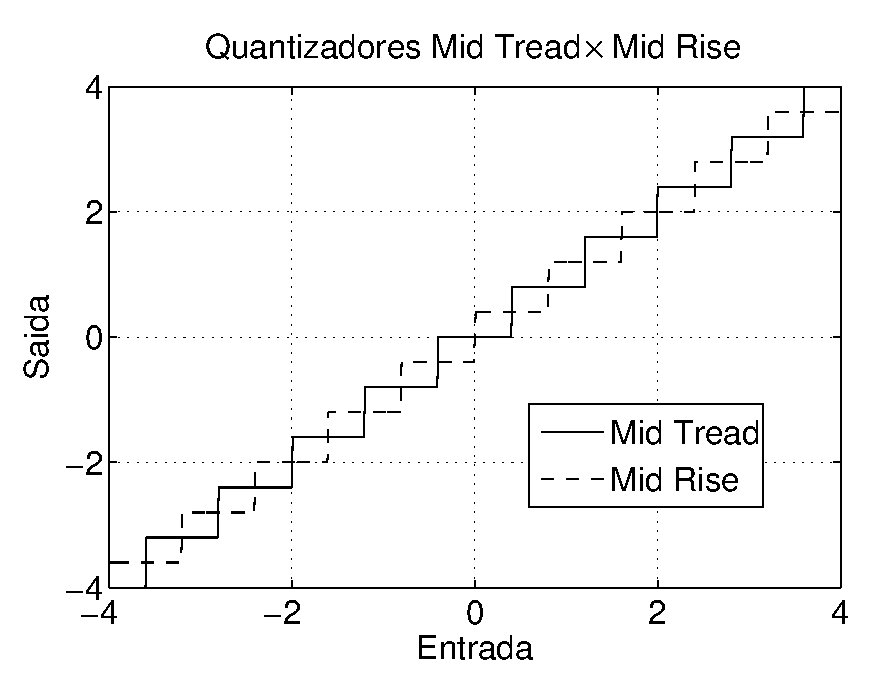
\includegraphics[width=7cm]{./quants.eps}}
\caption{Quantizador Midrise $\times$ Midtread.}\label{fig:quants}
\end{center}
\end{figure}

\end{itemize}

\item \textbf{Pergunta:} O que você observa? Quais são as diferenças entre os dois quantizadores?

\item \textbf{Tarefa:} Quantize a imagem Lena com os dois quantizadores acima e diferentes passos de quantização $2^n$ com $n\in {1,2,3,4,5}$ (assumindo que os pixeis estão entre 0 e 255, no caso de pixeis entre 0 e 1, faça as adequações necessárias). 

\item \textbf{Pergunta:} Para um mesmo $n$, há diferença visível entre as diferentes versões quantizadas das imagens? 

\item \textbf{Pergunta:} E quanto ao desempenho dos dois quantizadores em termos do erro introduzido pela quantização? Explique-os considerando os valores dos erros médios quadráticos obtidos para cada um e os gráficos dos erros de quantização.

\item \textbf{Tarefa:} Compare os histogramas correspondentes aos valoes dos pixeis da imagem original e os das quantizadas com os dois diferentes quantizadores com $n={2,4,6}$. 

\item \textbf{Tarefa:} Avalie as entropias dos pixeis nos sete casos. 

\item \textbf{Pergunta:} O que você conclui dos itens acima?

\end{enumerate}

\end{document}



